\documentclass[12pt,a4paper]{article}
\usepackage{ctex}
\usepackage{amsmath,amscd,amsbsy,amssymb,latexsym,url,bm,amsthm}
\usepackage{epsfig,graphicx,subfigure}
\usepackage{enumitem,balance}
\usepackage{wrapfig}
\usepackage{mathrsfs,euscript}
\usepackage[usenames]{xcolor}
\usepackage{hyperref}
\usepackage{caption}
\usepackage[vlined,ruled,linesnumbered]{algorithm2e}
\hypersetup{colorlinks=true,linkcolor=black}

\newtheorem{theorem}{Theorem}
\newtheorem{lemma}[theorem]{Lemma}
\newtheorem{proposition}[theorem]{Proposition}
\newtheorem{corollary}[theorem]{Corollary}
\newtheorem{exercise}{Exercise}
\newtheorem*{solution}{Solution}
\newtheorem{definition}{Definition}
\theoremstyle{definition}

\renewcommand{\thefootnote}{\fnsymbol{footnote}}

\newcommand{\postscript}[2]
 {\setlength{\epsfxsize}{#2\hsize}
  \centerline{\epsfbox{#1}}}

\renewcommand{\baselinestretch}{1.0}

\setlength{\oddsidemargin}{-0.365in}
\setlength{\evensidemargin}{-0.365in}
\setlength{\topmargin}{-0.3in}
\setlength{\headheight}{0in}
\setlength{\headsep}{0in}
\setlength{\textheight}{10.1in}
\setlength{\textwidth}{7in}
\makeatletter \renewenvironment{proof}[1][Proof] {\par\pushQED{\qed}\normalfont\topsep6\p@\@plus6\p@\relax\trivlist\item[\hskip\labelsep\bfseries#1\@addpunct{.}]\ignorespaces}{\popQED\endtrivlist\@endpefalse} \makeatother
\makeatletter
\renewenvironment{solution}[1][Solution] {\par\pushQED{\qed}\normalfont\topsep6\p@\@plus6\p@\relax\trivlist\item[\hskip\labelsep\bfseries#1\@addpunct{.}]\ignorespaces}{\popQED\endtrivlist\@endpefalse} \makeatother

\begin{document}
\captionsetup[figure]{labelfont={bf},labelformat={default},labelsep=period,name={Fig.}}

\noindent

%========================================================================
\noindent\framebox[\linewidth]{\shortstack[c]{
\Large{\textbf{Lab08-Graph Exploration}}\vspace{1mm}\\
CS214-Algorithm and Complexity, Xiaofeng Gao, Spring 2020.}}
\begin{center}
\footnotesize{\color{red}$*$ If there is any problem, please contact TA Yiming Liu.}

% Please write down your name, student id and email.
\footnotesize{\color{blue}$*$ Name: HaotianXue \quad Student ID:518021910506 \quad Email: xavihart@sjtu.edu.cn}
\end{center}

\begin{enumerate}
    \item
    \textbf{BFS Tree.} Similar to DFS, BFS yields a tree, (also possibly forest, but \textbf{just consider a tree} in this question) and we can define \textbf{tree, forward, back, cross} edges for BFS. Denote $Dist(u)$ as the distance between node $u$ and the source node in the BFS tree. Please prove:
    \begin{enumerate}
    	\item For both undirected and directed graphs, no forward edges exist in the graph.
    	
    	\item There are no back edges in undirected graph, while in directed graph each back edge $(u,v)$ yields $0\leq Dist(v)\leq Dist(u)$.
    	
    	\item For undirected graph, each cross edge $(u,v)$ yields $|Dist(v)-Dist(u)|\le 1$, while for directed graph, each cross edge $(u,v)$ yields $Dist(v)\leq Dist(u)+1$.
    	
    \end{enumerate}

   \begin{solution}
	  The solutions for problem1 is as follows.

	  We note the vertex with a longer distance as a deeper vertex in BFS tree.
	  
	  

	  (a) If there exists a forward edge from $u$ to $v$ in the BFS tree, then $y$ is a descendant but not a child of $u$ in BFS tree. 
	  It can never happen since BFS makes each neighbour of $u$ be explored after $u$ or before $u$. It means that $v$ can not 
	  have a distance more than $Dist(u) + 1$, so there has no forward edges in the tree.  
	  
	  (b)

	  \textbf{Undirected Graph:} When doing BFS in the undirected graph, if there exists one back edges $(u, v)$, where $v$ is an ancestor of $u$,
	  since $u,v$ are connected, $v$ can explore $u$ before $u$ tries to explore $v$, which contradicts the fact that $u$ is visiting $v$.
	  
	  \textbf{Directed Graph:} Since $v$ is an ancestor of $u$ , then $v$ is explored earlier than $u$. In BFS, it is obvious that the vertecx explored
	  earlier has a shorter distance that the distance of vertices explored later. So in the back edge we must have $Dist(v) \leq Dist(u)$.

	   (c)
	   Firstly, for \textbf{both undirected graph and directed graph}, $Dist(v) \leq Dist(u) + 1$. Since if $Dist(v) > Dist(u) + 1$, we define the father of $v$ as $v_f$,
	   then $v_f$ is deeper than $u$, then $u$ will have visited $v$ before $v_f$. And this will cause an contradiction.
	   
	   Then for the \textbf{undirected graph}. If $Dist(v) < Dist(u) - 1$, we consider the father of $u$:$u_f$, which is deeper than $v$, so $v$ will visit $u$ before $u_f$, which makes contradiction.

	   So considering the cases above, we have: in undirected graph $|Dist(v)-Dist(u)|\le 1$, while in directed graph, each cross edge $(u,v)$ yields $Dist(v)\leq Dist(u)+1$.


	  

   \end{solution}





    \item 
    \textbf{Articulation Points, Bridges, and Biconnected Components.} Let $G=(V, E)$ be a connected, undirected graph. An articulation point of $G$ is a vertex whose removal disconnects $G$. A bridge of $G$ is an edge whose removal disconnects $G .$ A biconnected component of $G$ is a maximal set of edges such that any two edges in the set lie on a common simple cycle. Figure\ref{def} illustrates these definitions. We can determine articulation points, bridges, and biconnected components using depth-first search. Let $G_{\pi}=\left(V, E_{\pi}\right)$ be a depth-first tree of $G$. Please prove:
    
    \begin{enumerate}
    	\item The root of $G_{\pi}$ is an articulation point of $G$ if and only if it has at least two children in $G_{\pi}$.
    	\item An edge of $G$ is a bridge if and only if it does not lie on any simple cycle of $G$.
    	\item The biconnected components of $G$ partition the nonbridge edges of $G$.
    \end{enumerate}

	 \begin{figure}[htbp]
	 	
		\centering
		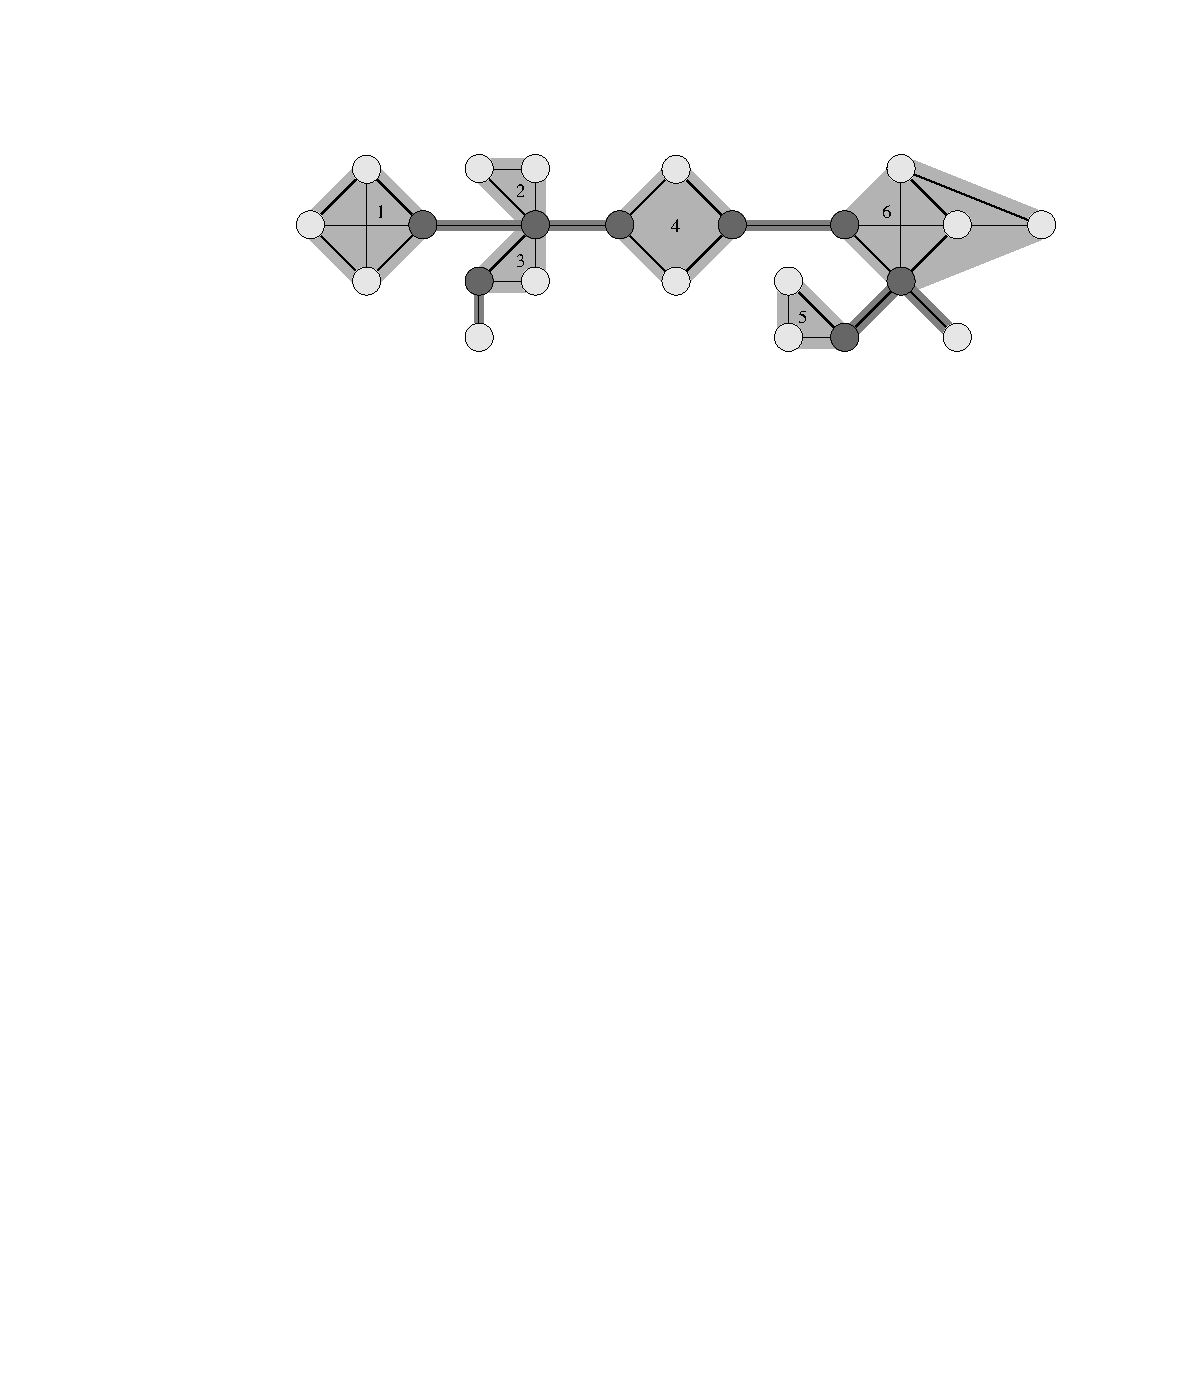
\includegraphics[width=6in]{Fig-Definition.pdf}
		\caption{The definition of articulation points, bridges, and biconnected components. The articulation points are the heavily shaded vertices, the bridges are the heavily shaded edges, and the biconnected components are the edges in the shaded regions, with a \textit{bcc} numbering shown.}
		\label{def}
	\end{figure}
	 
	\begin{solution}
	The solutions for this problem is as follows.
	
	(a) If the root of $G_{\pi}$ : $r$ has no less than two children, they are$c_1, c_2,...c_k$, then the trees rooted by $c_i$ is $T_i$. It is easy to prove that any two vertices  
$v_1$ in $T_i$ and $v_2$ in $T_j$, $v_1$ can only arrive $v_2$ through $r$, otherwise one of them can visit the other one, which makes them in the same tree.
So, if $r$ is removed from the graph, $G$ will become disconnected, then $r$ is an articulation point.

If $r$ is an articulation point, but $r$ has only one child(it is obvious that $r$ must have child). Then if $r$ is removed, we can explore from the child of $r$ and we can still 
visit the other vertices, which means $r$ is not an articulation point. So $r$ must have at least two children.

   (b)  If $e = (u,v)$ is an bridge of $G$ and $e$ is in a cycle of $G$.Then if we remove $e$, if a path between any two vertices $v_1$ and $v_2$ includes $e$, then it can move in the rest 
   of the cycle instead $e$. This shows that $G$ is still connected. So $e$ cannot be in a cycle.
   

   (c) According to (b), any edges in a cycle in $G$ cannot be a bridge of $G$, so any bridge in $G$ cannot be in
   a biconnected component. So the biconnected components partition the nonbridge edges in $G$.
   
   To be more strict, we can prove that biconnected component serves as a \textbf{Equivalence Class} for the vertices.
   And it is not difficult to prove that this relations satisfies the three properties:\textbf{reflesive, symmetric, transitive} for an equivalence class.
   We also know that Equivalence Class can make a partition of the original set. 

\end{solution}



    \item
    Suppose $G=(V, E)$ is a \textbf{Directed Acyclic Graph} (DAG) with positive weights $w(u, v)$ on each edge. Let $s$ be a vertex of $G$ with no incoming edges and assume that every other node is reachable from $s$ through some path.
    
    \begin{enumerate}
    	\item
    	Give an $O(|V|+|E|)$-time algorithm to compute the shortest paths from $s$ to all the other vertices in $G$. Note that this is faster than Dijkstra's algorithm in general.
    	\item
    	Give an efficient algorithm to compute the longest paths from $s$ to all the other vertices.
    \end{enumerate}
    
\end{enumerate}

\begin{solution}
The solution for this problem is as follows.

	(a)We can firstly use Topological Sorting to get a permutation of $E$ start from $s$. Then we visit the edges by the order in the list and update the distance, which 
	is shown in the pseudo code below:

\begin{minipage}[t]{0.90\textwidth}
	\begin{algorithm}[H]
		%\algsetup{footnotesize}
		%\scriptsize
		\KwIn{$G$, weight matrix$W$.}
		\KwOut{shortest path list $d[1, 2, ..., |V|]$}
		
		$d[s] = 0, d[i] = +\infty (i\neq s)$

		Calcualte the Topological Sorting list for $G$:$T=[s, v_1, v_2, .., v_k]$

		\For{$v$ in $T$}{
			\For{$(u, v)$ in $E$}{
			    $d[v]$ = $min(d[v], d[u] + W(u, v))$
			}
		}
	
		\Return{$d$}\;
		
	\end{algorithm}
\end{minipage}

(b)
We can actually turn all the weights $w$ into $-w$, then we can use (a) to solve the problem. 

\begin{minipage}[t]{0.90\textwidth}
	\begin{algorithm}[H]
		%\algsetup{footnotesize}
		%\scriptsize
		\KwIn{$G$, weight matrix$W$.}
		\KwOut{shortest path list $d[1, 2, ..., |V|]$}
		
		$W = -W$
		
		$d[s] = 0, d[i] = +\infty (i\neq s)$

		Calcualte the Topological Sorting list for $G$:$T=[s, v_1, v_2, .., v_k]$

		\For{$v$ in $T$}{
			\For{$(u, v)$ in $E$}{
			    $d[v]$ = $min(d[v], d[u] + W(u, v))$
			}
		}
	
		\Return{$-d$}\;
		
	\end{algorithm}
\end{minipage}

\end{solution}

\vspace{20pt}

\textbf{Remark:} You need to include your .pdf and .tex files in your uploaded .rar or .zip file.

%========================================================================
\end{document}
